% Report_draft.tex — LaTeX rendering of docs/progress/Report_draft.md
% Build (from this directory):
%   pdflatex -interaction=nonstopmode Report_draft.tex   (twice, for \ref)
% Images resolve through \graphicspath: the down-scaled build copies under
% ../../code/pics/pdfimg/ first, the full-resolution originals in
% ../../code/pics/ second. Remove pdfimg/ to render from the originals.
\documentclass[11pt,a4paper]{article}

\usepackage[T1]{fontenc}
\usepackage[utf8]{inputenc}
\usepackage{lmodern}   % scalable (Type 1) fonts, required by microtype expansion
\usepackage[a4paper,margin=2.5cm]{geometry}
\usepackage{graphicx}
\usepackage{booktabs}
\usepackage{tabularx}
\usepackage{array}
\usepackage{amsmath}
\usepackage{xcolor}
\usepackage{textcomp}
\usepackage{tikz}
\usetikzlibrary{arrows.meta,positioning}
\usepackage{caption}
\usepackage{float}
\usepackage{placeins}
\usepackage{placeins}
\usepackage{enumitem}
\usepackage{microtype}
\usepackage[hidelinks]{hyperref}

\graphicspath{{../../code/pics/pdfimg/}{../../code/pics/}}
% Figures are referenced WITHOUT an extension so the build resolves them in
% \graphicspath order: the down-scaled copy in pdfimg/ if present (the six
% photographic renders are .jpg there), otherwise the full-resolution original
% in code/pics/ (.png). Without this list the .jpg names would not fall back.
\DeclareGraphicsExtensions{.jpg,.jpeg,.png,.pdf}

\captionsetup{font=small,labelfont=bf,labelsep=period}
% Long file paths in \texttt{} are unbreakable and overflow the margin. \cpath
% adds \allowbreak after each / and _ so TeX can break a path at a natural
% separator when it would otherwise run past the margin. Implemented with expl3
% token lists so it is safe inside captions and other moving arguments.
\ExplSyntaxOn
\NewDocumentCommand{\cpath}{m}
  {
    \texttt
      {
        \group_begin:
        \tl_set:Nn \l_tmpa_tl {#1}
        \tl_replace_all:Nnn \l_tmpa_tl { / } { /\allowbreak{} }
        \tl_replace_all:Nnn \l_tmpa_tl { \_ } { \_\allowbreak{} }
        \tl_use:N \l_tmpa_tl
        \group_end:
      }
  }
\ExplSyntaxOff
\setlength{\parindent}{0pt}
\setlength{\parskip}{0.6em}
% let TeX stretch line spacing a little before overfull rather than overflowing
\setlength{\emergencystretch}{3em}
\renewcommand{\arraystretch}{1.15}
\setlist[itemize]{leftmargin=1.4em,itemsep=0.2em,topsep=0.3em}
% ragged-right the X (wrapping) columns so long table cells wrap instead of
% overfull, and use smaller gaps between columns
\renewcommand{\tabularxcolumn}[1]{p{#1}}
\newcolumntype{Y}{>{\raggedright\arraybackslash}X}

% full-width figure, aspect ratio locked
\newcommand{\figfull}[3]{%
  \begin{figure}[htbp]\centering
  \includegraphics[width=\textwidth,height=0.85\textheight,keepaspectratio]{#1}%
  \caption{#2}\label{#3}\end{figure}}
% figure constrained by height only (tall images)
\newcommand{\figtall}[3]{%
  \begin{figure}[htbp]\centering
  \includegraphics[height=0.70\textheight,keepaspectratio]{#1}%
  \caption{#2}\label{#3}\end{figure}}
% figure at a fraction of the text width: \figpart{width}{file}{caption}{label}
\newcommand{\figpart}[4]{%
  \begin{figure}[htbp]\centering
  \includegraphics[width=#1\textwidth,height=0.85\textheight,keepaspectratio]{#2}%
  \caption{#3}\label{#4}\end{figure}}
% 2x2 comparison grids: slightly inset so two consecutive grids can share a page
\newcommand{\figgrid}[3]{%
  \begin{figure}[htbp]\centering
  \includegraphics[width=0.95\textwidth,height=0.85\textheight,keepaspectratio]{#1}%
  \caption{#2}\label{#3}\end{figure}}

\begin{document}

\begin{center}
{\Large\bfseries COMP4423 -- Assignment 1\\
Triangle-Brick Image Generation\par}
\vspace{0.6em}
{\normalsize Huang Haoran (24101322D)\par}
\vspace{0.2em}
{\small\textbf{Repository:}\ \url{https://github.com/Retr0-rgb-lab/COMP4423_Assignment1}\par}
\end{center}

\FloatBarrier
\FloatBarrier
\section{Introduction}

Given a single image, the assignment asks to convert it into a mosaic of
triangular bricks that visually approximates the original, under a hard budget
of at most 10{,}000 individual right-isosceles triangles, with no gaps or
overlaps, where each brick carries one uniform face colour determined from the
image region it covers. Multiple brick sizes and multiple colours are allowed.

The no-gaps/no-overlaps rule is a hard constraint, so I did not want to rest it
on the construction argument alone. \texttt{code/verify\_coverage.py} checks it
directly for all three delivered tessellations: cells are distinct and
grid-aligned, each cell's two triangles satisfy the exact area identity
$\mathrm{area}(a) + \mathrm{area}(b) = s^{2}$ (shoelace on the vertices), and
rasterising the triangles leaves \textbf{0 uncovered pixels} in the delivered
crop. The test is geometric rather than a rasterised multiplicity count because
\texttt{cv2.fillPoly} paints a one-pixel fringe along every internal diagonal ---
a rasterisation convention, not an area overlap, and one I quantify separately in
Section~\ref{sec:t2-problems}. All three pass.

Because the budget is fixed, the real work is deciding where the detail should
go. More triangles capture more edges and texture, but they also make each
brick's colour estimate noisier (a tiny triangle averages very few pixels, so
sensor noise starts to look like detail), and none of that addresses the colour
error introduced by mapping each region to a fixed palette entry. I treat the
three as separate things and let each task attack whichever matters most at
that point.

I built the system in four stages, and each stage surfaced a problem that
shaped the next. Task 2 fixes the tessellation to equal-size bricks with three
colours; measuring its output showed that a uniform grid does not align with
image content, which became the motivation for Task 3. Task 3 makes both the
geometry and the palette adaptive, which is where the budget-allocation
question above is actually answered. Task 4 runs the same pipeline in a live
camera loop, where the speed and stability problems the offline setting hides
become the main engineering work.

\textbf{Test image.} The test photo for this report is
\texttt{code/pics/sky.jpg} (1706$\times$1279), a canal-side cityscape --- brick
wall, trees, distant buildings --- captured on the camera used for Task 1. Its
dominant signal is luminance variation rather than hue variation, which has a
measurable effect on the colour-quantisation experiments (Sections~\ref{sec:t2}
and~\ref{sec:t3}).

\figfull{sky}{The test photo \texttt{code/pics/sky.jpg}
(1706$\times$1279): a canal-side cityscape with brick architecture, trees and
distant buildings.}{fig:testphoto}

\FloatBarrier
\FloatBarrier
\section{Task 1 --- capture and display}

Task 1 is to call the camera, capture a frame, and display it. The program is
\texttt{code/capture.py}: it opens the default camera with
\texttt{cv2.VideoCapture(0)}, reads one frame, prints its shape and channel
order, and shows it with \texttt{cv2.imshow} until a key is pressed, at which
point the capture is released and the window closed. Running it on the machine
with the camera attached:

\begin{verbatim}
python code\capture.py
\end{verbatim}

That is the Task 1 deliverable in full. The script also accepts
\texttt{--from-file PATH} to read a still frame instead of opening a camera, and
\texttt{--save PATH} to write the frame to disk, both of which let the capture
path be exercised and inspected without a live camera in front of it. The frame
shown in Fig.~\ref{fig:testphoto} is the test photo this report works from.

\FloatBarrier
\FloatBarrier
\section{Method --- the shared toolkit}

The four tasks share one geometry, colour and rendering core
(\texttt{code/brick\_geom.py}, \texttt{brick\_color.py},
\texttt{brick\_render.py}, \texttt{brick\_metrics.py}). I kept the decisions
that every task depends on in this one place, so later sections only have to
add the one thing each task changes. Table~\ref{tab:toolkit} summarises them.

\begin{table}[htbp]
\centering
\footnotesize
\begin{tabularx}{\textwidth}{@{}p{2.6cm}Y Y@{}}
\toprule
\textbf{Component} & \textbf{Choice} & \textbf{Rationale}\\
\midrule
Brick geometry
  & Square cell cut by \textbf{one diagonal}, direction alternates by checkerboard parity
  & Guarantees right-isosceles, gap-free, overlap-free tiling; alternation avoids a visible single-directional smear\\
Brick size
  & Length of the equal legs, in base-grid units; Task 2 fixed, Task 3 power-of-two sizes \{1,2,4,8,16,32,\ldots\}
  & PDF definition; powers of two make quadtree halving exact\\
Colour per brick
  & Mean BGR of the pixels under the triangle's mask (\texttt{cv2.fillPoly} + \texttt{cv2.mean})
  & Robust to sub-region detail; the PDF asks colour be determined from the region covered\\
Palette (Task 2)
  & \textbf{Multi-Otsu on BT.601 luminance} (primary), K-Means $K=3$ and a fixed 33\%/67\% percentile split as baselines
  & Otsu thresholds adapt to the scene histogram; baselines make the results section a real comparison\\
Palette (Task 3)
  & \textbf{K-Means on CIE-Lab} ($K=8/16$), Median-Cut as baseline
  & Lab is perceptually uniform; median cut is cheap and deterministic\\
Tessellation (Task 3)
  & \textbf{Top-down RDO quadtree}, split priority $\Delta$MSE per triangle ($\Delta$SSE/6); region-merge as dual algorithm
  & Rate--distortion allocation: equal per-triangle units make different sizes comparable\\
Border
  & 1-px \texttt{\#3C3C3C} polyline per triangle
  & Visual separation; PDF permits drawn boundaries, not counted as brick colours\\
Metrics
  & 10-item metric suite (9 quality + 1 constraint): PSNR, SSIM, MS-SSIM (4-level mean, a practical variant of Wang et al. multi-scale SSIM), $\Delta$E2000 (CIEDE2000), Edge F1/Precision/Recall (Canny + 3-px tolerance), \textbf{edge-alignment correlation (EAC; Pearson correlation of Sobel responses --- labelled ``EPI'' below for short)}, Quantisation Error, Budget Utilisation
  & Each metric catches a different failure mode; the EAC/EPI metric specifically measures whether triangle boundaries align with real edges\\
\bottomrule
\end{tabularx}
\caption{Design decisions of the shared geometry/colour/rendering toolkit.}
\label{tab:toolkit}
\end{table}

\textbf{Budget semantics.} The limit is 10{,}000 \emph{triangles} (``bricks''); a
quadtree leaf cell produces 2 triangles, so a partition of 4{,}995 cells
exhausts the budget at 9{,}990 triangles. All Task 3 runs use
9{,}988--9{,}990 triangles, which is 99.88--99.90\% of the budget.

\textbf{Metric evaluation region.} All PSNR/SSIM/$\Delta$E/Edge/EPI numbers in
Sections~\ref{sec:t2}--\ref{sec:t3} are computed on the rendered canvas with the
1-px border drawn. The border is \texttt{\#3C3C3C} and, on the chosen Task 3
render, covers 11.6\% of pixels, so it is a constant confound shared by every
run; its effect is quantified in Section~\ref{sec:chosen-config}. The 9 quality
metrics are PSNR, SSIM, MS-SSIM, $\Delta$E2000, Edge F1/Precision/Recall, EPI
and Quantisation Error, with Budget Utilisation tracked separately as a
constraint. Appendix~\ref{app:metrics} gives the exact definition and the
direction of each one, because several of them disagree with each other on
purpose.

\FloatBarrier
\FloatBarrier
\section{Task 2 --- equal-size triangles, 3 colours}
\label{sec:t2}

\FloatBarrier
\FloatBarrier
\subsection{Design and testing}

The tessellation is a uniform $S\times S$ grid cut by checkerboard diagonals. The
grid step is the smallest $S$ for which $2\cdot M\cdot N \leq 10000$
($M=\lceil H/S\rceil$, $N=\lceil W/S\rceil$). For the three colours I compare
three quantisation methods on identical geometry and means. The primary one is
Multi-Otsu: an exhaustive two-threshold search over the BT.601 luminance
histogram, with each class painted the mean BGR of its members. As baselines I
also run K-Means with $K=3$ on BGR (K-Means++ initialisation) and a fixed
percentile split at 33\%/67\% of the luminance histogram, the last being a
deliberately naive baseline that ignores scene statistics entirely.

\emph{How it was tested.} All three share one geometry (59$\times$78, $S=22$,
9{,}204 triangles on \texttt{sky.jpg}) so only the quantiser differs; the full
10-item metric suite is computed per method. Outputs:
\cpath{code/pics/task2/out\_task2\_compare.png} (original + 3 renders),
\texttt{out\_task2\_residual.png} (per-pixel $\Delta$E2000 heatmaps),
\texttt{out\_task2\_metrics\_chart.png}.

\FloatBarrier
\FloatBarrier
\subsection{Results}

\begin{table}[htbp]
\centering
\begin{tabular}{@{}l r r r@{}}
\toprule
\textbf{Metric} & \textbf{otsu} & \textbf{kmeans} & \textbf{fixed}\\
\midrule
PSNR up (dB)           & 16.15 & 16.16 & 15.58 \\
SSIM up                & 0.332 & 0.334 & 0.286 \\
MS-SSIM up             & 0.482 & 0.481 & 0.452 \\
$\Delta$E2000 down     & 11.41 & 11.41 & 11.92 \\
Edge F1 up             & 0.191 & 0.189 & \textbf{0.233} \\
Edge Precision up      & 0.151 & 0.150 & 0.171 \\
Edge Recall up         & 0.261 & 0.255 & \textbf{0.365} \\
EPI up                 & -0.028 & -0.031 & -0.012 \\
Quant Error down       & 8.47 & 8.48 & 8.98 \\
\bottomrule
\end{tabular}
\caption{Task 2 results: three colour quantisers on identical geometry
(59$\times$78, $S=22$, 9{,}204 triangles, \texttt{sky.jpg}).}
\label{tab:t2}
\end{table}

Three things stand out in this table. First, otsu and kmeans are
indistinguishable on this scene: the palettes differ by at most 2 per channel
and SSIM by only 0.002 (0.332 vs 0.334). K-Means in 3-D BGR is collapsing onto
the same 1-D luminance split that Multi-Otsu uses directly, because the
dominant signal here is luminance, not hue; its theoretical colour-resolution
advantage never shows up on a near-grayscale image.

Second, and more interesting, \texttt{fixed} wins on every edge metric while
losing on every colour and structure metric. Its uniform 33\%/67\% thresholds
happen to place more of the original edges exactly on a colour boundary between
adjacent triangles, so those edges survive as hard boundaries. Otsu and K-Means
push their thresholds to perceptually meaningful splits (sky versus wall) and
instead smooth over thin edges. There is a real trade-off here between
perceptual fidelity and raw edge preservation, and which method is ``better''
depends on what one means by quality.

Third, EPI is negative for all three methods (about $-0.03$). A negative EPI
means the output has weak edges where the original has strong ones and vice
versa: the regular grid is introducing boundaries that have nothing to do with
the image content. That is the quantitative signature of the uniform grid's
geometric mismatch, and it is the main reason I move to an adaptive
tessellation in Task 3.

\figgrid{task2/out_task2_compare}{Task 2 comparison grid: the original image
and the three colour-quantisation results (Multi-Otsu, K-Means, fixed
percentile) on identical geometry, with their key metrics. \texttt{fixed}
visibly collapses the sky into a mid-grey band (its 33\%/67\% split ignores
scene statistics).}{fig:t2compare}

\figtall{task2/out_task2_residual}{Per-pixel $\Delta$E2000 residual heatmaps
(JET, blue = small error) for the three quantisers. Otsu and K-Means are nearly
identical with error concentrated in tree foliage; \texttt{fixed} adds a bright
error band across the water.}{fig:t2residual}

\figpart{0.92}{task2/out_task2_metrics_chart}{Task 2 metric summary across
the three quantisers (normalised and absolute scales). Otsu $\approx$ K-Means on
colour/structure; \texttt{fixed} wins only the edge family.}{fig:t2chart}

\FloatBarrier
\FloatBarrier
\subsection{Problems found and solved}
\label{sec:t2-problems}

The first run produced only two triangles because \texttt{compute\_grid} scanned
$S$ downward and returned the largest $S$ that fit the budget, which for this
image is a 1$\times$1 grid. The code was syntactically valid but semantically
wrong; the loop has to grow $S$ upward and return the smallest $S$ that stays
under budget. I fixed it by inverting the scan
(\cpath{code/brick\_geom.py::compute\_grid}).

The grid also left a black band. The floor-based grid dropped the trailing rows
and columns that did not form a full $S\times S$ square (5\,px on the right,
19\,px on the bottom of \texttt{sky.jpg}), so those pixels stayed black and
inflated the PSNR/SSIM error. I fixed this by switching to a \texttt{ceil} grid
and reflect-padding the image to $M\cdot S \times N\cdot S$, rendering, then
cropping back to the original size
(\cpath{code/triangle\_brick.py::preprocess}). After the fix SSIM rises from
0.3226 to 0.3316 and PSNR from 15.76 to 16.15\,dB; the pre-fix numbers are
preserved in git at commit \texttt{a5d2d76} if a direct before/after is needed.

The grid-selection bug came from an AI-written draft: the model produced the
\texttt{compute\_grid} loop with the scan direction inverted, the code was
syntactically valid, and only a manual pass through the logic --- tracing what
the loop returns for a large image --- showed it was wrong. I corrected it by
hand. That episode is a reminder that AI-generated logic is not guaranteed to
be correct, and that every such function needs its control flow checked step by
step rather than trusted because it runs.

\FloatBarrier
\FloatBarrier
\section{Task 3 --- adaptive multi-size, multi-colour}
\label{sec:t3}

\FloatBarrier
\FloatBarrier
\subsection{Design and testing}

I built on Task 2 by adding two adaptive pieces. The tessellation is now a
\textbf{top-down RDO quadtree} that starts from a coarse grid and splits the
highest-priority cell ($\Delta$MSE/6) while budget remains, and the palette is
now \textbf{K-Means-Lab} with $K>3$, with Median-Cut kept as a baseline. I
dropped the Task 2 primary quantiser (Multi-Otsu) because Otsu is a 1-D
luminance method that cannot produce more than a small number of threshold
classes. Task 3 needs an arbitrary $K$-colour palette, so I replaced it with a
general clustering method on the perceptually uniform Lab space.

\textbf{Region merging (dual algorithm).} As a contrast to the top-down
quadtree, I also implemented a bottom-up region-merge
(\texttt{brick\_region\_merge}). It starts from cells of the smallest allowed
size and greedily merges an aligned 2$\times$2 block of equal-size cells into
one cell of twice the side while the triangle budget allows, using summed-area
tables to score each merge candidate. The merge candidates are generated on the
\texttt{target\_size} grid so every merged block can itself form the next
level's 2$\times$2 block. On \texttt{sky.jpg} it terminates at 9{,}990 triangles
with 44{,}415 merges and a final size distribution of only \{16,32\} (it merges
all fine cells away), which is the property that drives its comparison against
the quadtree in Section~\ref{sec:t3-results}.

I designed a 15-run experiment grid that changes one variable at a time and
holds everything else fixed, so that any difference in the metrics can be
attributed to that one variable. Each group answers a specific design question:

\begin{table}[htbp]
\centering
\footnotesize
\begin{tabularx}{\textwidth}{@{}l Y Y@{}}
\toprule
\textbf{group} & \textbf{changed variable (everything else fixed)} & \textbf{the design question it answers}\\
\midrule
\texttt{A\_ksweep}   & $K \in \{4, 8, 16\}$ & Does a larger palette improve colour error, and at what cost to structure?\\
\texttt{B\_sweep}    & $S_{\min} \in \{2, 4, 8\}$ (..32) & Does dropping the smallest cells from the allowed set matter?\\
\texttt{B2\_smax}    & $S_{\max} \in \{32, 64, 128\}$ & Does starting from a coarser grid (more budget headroom for deep splits) change the result?\\
\texttt{C\_algorithm}& partition: quadtree vs region-merge & Which tessellation strategy --- top-down RDO or bottom-up merging --- is better?\\
\texttt{D\_palette}  & palette: K-Means-Lab vs Median-Cut & Which palette method, with geometry fixed, wins on colour and on structure?\\
\texttt{E\_priority} & priority: $\Delta$MSE vs Sobel edge-density & Does the split priority affect edge alignment, or is $\Delta$MSE the right choice?\\
\bottomrule
\end{tabularx}
\end{table}

All runs use 9{,}988--9{,}990 triangles, i.e. 99.88--99.90\% of the budget. The
full table is at \cpath{code/pics/task3/summary/metrics\_table.csv}.

\FloatBarrier
\FloatBarrier
\subsection{Results (selected rows)}
\label{sec:t3-results}

\begin{table}[htbp]
\centering
\footnotesize
\setlength{\tabcolsep}{4pt}
\begin{tabular}{@{}l r r r r r r@{}}
\toprule
\textbf{run} & \textbf{SSIM up} & \textbf{MS-SSIM up} & \textbf{$\Delta$E2000 down} & \textbf{Edge F1 up} & \textbf{EPI up} & \textbf{Quant Err down}\\
\midrule
A:k04                  & \textbf{0.384} & 0.513 & 11.08 & 0.330 & \textbf{0.064} & 9.25 \\
A:k16                  & 0.360 & \textbf{0.539} & \textbf{8.74} & 0.348 & 0.047 & \textbf{5.62} \\
B2:smax\_32            & 0.359 & 0.520 & \textbf{9.95} & 0.295 & 0.046 & 7.30 \\
\textbf{B2:smax\_64}   & \textbf{0.421} & \textbf{0.555} & 10.21 & \textbf{0.377} & \textbf{0.109} & 7.41 \\
C:quadtree             & 0.359 & 0.520 & 9.95 & 0.295 & 0.046 & 7.30 \\
C:region\_merge        & 0.332 & 0.522 & \textbf{9.59} & 0.298 & 0.019 & \textbf{6.47} \\
D:median\_cut          & 0.375 & 0.526 & 10.61 & 0.322 & 0.052 & 7.76 \\
E:prio\_mse            & 0.370 & 0.518 & 10.22 & 0.320 & 0.050 & 7.33 \\
E:prio\_edgef1         & 0.374 & 0.499 & 9.83 & \textbf{0.213} & \textbf{-0.020} & 6.45 \\
\bottomrule
\end{tabular}
\caption{Task 3 results (selected rows of the 15-run sweep; source
\texttt{metrics\_table.csv}).}
\label{tab:t3}
\end{table}

\emph{(The rows \texttt{C:quadtree}, \texttt{B2:smax\_32} and
\texttt{D:kmeans\_lab} are the same default run of the same configuration and
reproduce the same values (SSIM 0.359, $\Delta$E 9.95); \texttt{E:prio\_mse}
shares the configuration but differs slightly (SSIM 0.370) because K-Means-Lab
is run-to-run non-reproducible (Section~\ref{sec:chosen-config}). The full
15-row table is in \cpath{code/pics/task3/summary/metrics\_table.csv}.)}

\emph{(Provenance note for the \texttt{E:prio\_edgef1} row: its numbers were
recorded on the original per-region Sobel reference path. The current
\texttt{impl="sat"} runs Sobel once globally and gives values that differ near
region edges (median $\sim$2$\times$ relative difference), so this exact row is
not reproducible from the shipped code; the verdict below is robust under both
implementations.)}

\textbf{Noise audit --- which of these rows can carry a conclusion.} Thirteen of
the fifteen rows use K-Means-Lab, and that sweep driver never seeds OpenCV's RNG,
so each row is a single unseeded draw. I measured the resulting spread instead of
assuming it. Four consecutive runs of one fixed configuration (quadtree,
$S_{\text{set}}=[1..32]$, $K=8$, 9{,}990 triangles) returned:

\begin{table}[htbp]
\centering
\begin{tabular}{@{}l r r r r r@{}}
\toprule
\textbf{metric} & \textbf{run 1} & \textbf{run 2} & \textbf{run 3} & \textbf{run 4} & \textbf{spread}\\
\midrule
$\Delta$E2000 & 10.2519 & 9.8111 & 9.9255 & 9.8406 & \textbf{0.441} \\
SSIM         & 0.36675 & 0.36030 & 0.36020 & 0.36405 & \textbf{0.0066} \\
Edge F1      & 0.32247 & 0.30441 & 0.31731 & 0.29387 & \textbf{0.029} \\
EPI          & +0.04740 & +0.04555 & +0.04731 & +0.04762 & \textbf{0.0021} \\
Quant Error  & 7.30 & 7.76 & 7.38 & 7.46 & \textbf{0.178} \\
\bottomrule
\end{tabular}
\end{table}

The geometry is deterministic across all four runs (identical 4{,}995-cell
partition); only the palette moves, and eight palette builds on \emph{frozen}
geometry returned eight distinct palettes. So each metric has its own noise
floor, and a gap only means something when it is large relative to \emph{that
metric's} floor. Comparing a $\Delta$E2000 gap against an Edge F1 gap would not
be valid, so the table below uses the matching floor:

\begin{table}[htbp]
\centering
\footnotesize
\begin{tabular}{@{}l l r r r l@{}}
\toprule
\textbf{comparison} & \textbf{metric} & \textbf{gap} & \textbf{floor} & \textbf{ratio} & \textbf{verdict}\\
\midrule
K sweep, K=4 $\rightarrow$ 16                       & $\Delta$E2000 & 2.340 & 0.441 & 5.3x & load-bearing \\
$S_{\max}$ 32 $\rightarrow$ 64                     & SSIM         & 0.062 & 0.0066 & 9.5x & load-bearing \\
$S_{\max}$ 32 $\rightarrow$ 64                     & Edge F1      & 0.082 & 0.029 & 2.9x & load-bearing \\
priority, $\Delta$MSE $\rightarrow$ Sobel          & EPI          & 0.070 & 0.0021 & 34x & load-bearing \\
priority, $\Delta$MSE $\rightarrow$ Sobel          & Edge F1      & 0.107 & 0.029 & 3.7x & load-bearing \\
quadtree vs region-merge                          & EPI          & 0.027 & 0.0021 & 13x & load-bearing \\
quadtree vs region-merge                          & SSIM         & 0.027 & 0.0066 & 4.1x & load-bearing \\
palette, K-Means-Lab vs Median-Cut                & $\Delta$E2000 & 0.660 & 0.441 & 1.5x & \textbf{marginal --- see below} \\
$S_{\max}$ 32 $\rightarrow$ 64                     & $\Delta$E2000 & 0.260 & 0.441 & 0.6x & inside noise \\
$S_{\max}$ 64 $\rightarrow$ 128                    & $\Delta$E2000 & 0.069 & 0.441 & 0.2x & inside noise \\
priority, $\Delta$MSE $\rightarrow$ Sobel          & $\Delta$E2000 & 0.390 & 0.441 & 0.9x & inside noise \\
\bottomrule
\end{tabular}
\end{table}

So four of the comparisons I draw conclusions from clear their own metric's
floor by 2.9$\times$ or better, and three do not. Where a conclusion needed the
colour side, I re-ran it with a deterministic palette --- that is what
Section~\ref{sec:smax-tradeoff} does, and there the $\Delta$E2000 gap is
10.61 $\rightarrow$ 11.77 (spread 1.16, 2.6$\times$ the floor). The
quadtree-vs-region-merge colour verdict in Section~\ref{sec:chosen-config} is
taken from the \emph{seeded} Table~\ref{tab:chosen}, which makes it
reproducible, though at $+0.32$ it is still inside the colour floor; that
decision rests on the structure gap instead, as Section~\ref{sec:chosen-config}
states. The palette comparison is the interesting borderline case, and I treat it
explicitly in Section~\ref{sec:chosen-config} rather than claiming it as a win.

Key findings (all on the single test image \texttt{sky.jpg}):

\begin{quote}
\textbf{Tying back to Task 2's motivation.} Section~\ref{sec:t2} reported a
negative EPI ($\approx -0.03$) for the uniform grid and used it as the
motivation for adaptive geometry. The adaptive configuration now makes EPI
positive for the chosen config ($+0.045$, Section~\ref{sec:chosen-config}) and
it rises to $+0.109$ at $S_{\max}=64$, while Task 2's best Edge F1 was 0.233
(the fixed-percentile quantiser). (The two families are not directly
comparable: 3 colours vs 16, 9{,}204 vs 9{,}990 bricks, but the direction of
the change is the one I was after.)
\end{quote}

Larger $K$ monotonically improves colour error. From $K=4$ to $K=16$,
$\Delta$E2000 moves from 11.08 to 8.74 and Quant from 9.25 to 5.62, at a small
structure cost (SSIM 0.384 to 0.360). \textbf{$K=16$} minimises colour error, but
the best SSIM and EPI of the $K$ sweep both belong to $K=4$ (0.384 and 0.064),
so the chosen config is a balanced compromise.

Raising $S_{\max}$ from 32 to 64 was the largest structure and edge win of the
sweep: SSIM moved from 0.359 to 0.421, MS-SSIM from 0.520 to 0.555, Edge F1 from
0.295 to 0.377, and EPI from 0.046 to 0.109 (more than doubled). A coarser start
grid leaves more budget for the deep splits where detail matters. The matching
$\Delta$E2000 move is 9.95 $\rightarrow$ 10.21, a $+2.6\%$ regression, but that
particular gap is smaller than this sweep's $\sim$0.4 noise floor, so I treat the
colour side as unresolved here and establish it deterministically in
Section~\ref{sec:smax-tradeoff} instead. Going to $S_{\max}=128$ changes every
structural metric by less than 0.01 against 64 (SSIM 0.423 vs 0.421, Edge F1
0.378 vs 0.377) and ends two triangles under budget at 9{,}988; the colour-side
columns move slightly more ($\Delta$E2000 0.069, Quant Error 0.029, PSNR
0.014\,dB) but all of those gaps are an order of magnitude inside the $\sim$0.4
noise floor, so the defensible statement is only that 128 buys nothing
measurable over 64.

$\Delta$MSE priority is the better choice on the edge-alignment metrics. The
Sobel version is the only negative-EPI run of the grid ($-0.020$) and has by far
the worst Edge F1 (0.213 against 0.320), which is the failure that matters here
because it means the triangle boundaries stopped following image structure. Both
of those gaps are far outside the noise floor, and they are what the choice
rests on. Sobel does lead on several colour-side scores ($\Delta$E2000 9.83 vs
10.22, Quant Error 6.45 vs 7.33, SSIM 0.374 vs 0.370), but those gaps sit inside
the noise, so the honest summary is that edge-density allocation over-exploits
high-gradient pixels without aligning boundaries to real edges, with no
measurable colour-side benefit. The measurements largely rejected this otherwise
plausible-sounding suggestion.

Comparing quadtree against region-merge, the quadtree wins on structure (SSIM
0.359 vs 0.332, EPI $+0.046$ vs $+0.019$) while region-merge leads on the colour
columns ($\Delta$E2000 9.59 vs 9.95). The structure gap is well outside the noise;
the colour gap of 0.36 is not, so I take that verdict from the seeded comparison in
Section~\ref{sec:chosen-config} instead. Either way the mechanism is the same and
is not in doubt: region-merge collapses to only \{16,32\} cells, while the
quadtree keeps a \{4,8,16,32\} mix.

\figfull{task3/summary/metrics_chart}{All 15 Task 3 runs as a per-metric bar
chart. The x-axis of each panel carries the metrics (left: the four
$[0,1]$-bounded scores; right: the absolute-scale ones), and the 15 runs are
series within each group, identified by the legend, which is where the swept
variable ($K$, $S_{\text{set}}$, partition, palette, priority) shows up. The
structural-vs-colour split is visible across the whole grid.}{fig:t3chart}

\FloatBarrier
\FloatBarrier
\subsection{The marginal-benefit / rate-distortion study}

Driving $S_{\max}$ upward raised a question I wanted to answer: at what size does
splitting stop paying? I ran a dedicated experiment with a 60{,}000-triangle
budget that recorded each split's marginal benefit ($\Delta$SSE per new triangle)
by parent size. Three figures, each from a different file in
\texttt{code/pics/task3/analysis/}, show the three sides of the answer; the
numbers behind them are in Table~\ref{tab:marginal}.

\begin{table}[htbp]
\centering
\begin{tabular}{@{}l r r r@{}}
\toprule
\textbf{parent size} & \textbf{splits} & \textbf{mean $\Delta$SSE/tri} & \textbf{share of total benefit}\\
\midrule
64 & 484  & 345{,}760 & 39.3\% \\
32 & 972  & 111{,}064 & 25.4\% \\
16 & 1766 & 39{,}219  & 16.3\% \\
8  & 2964 & 16{,}889  & 11.8\% \\
4  & 3277 & 8{,}833   & 6.8\% \\
2  & 357  & 5{,}071   & 0.4\% \\
\bottomrule
\end{tabular}
\caption{Marginal benefit of a split by parent cell size (60{,}000-triangle
run).}
\label{tab:marginal}
\end{table}

\figpart{0.9}{task3/analysis/marginal_benefit_curve}{The marginal-benefit
curve (\texttt{marginal\_benefit\_curve.png}): each split's benefit,
$\Delta$SSE per new triangle, plotted in greedy split order on a log y-axis
against the running triangle count. The envelope decays from roughly
$6\times10^{6}$ at the first split to about $10^{4}$ at the tail; the red line
marks the 9{,}990 assignment budget, where a split still pays but the remaining
budget would only buy ever-smaller cells.}{fig:marginal}

\figpart{0.9}{task3/analysis/cumulative_benefit_curve}{The cumulative view
(\texttt{cumulative\_benefit\_curve.png}): the same split benefits added up,
normalised to the full 60{,}000-triangle total. Around three-quarters of the
total error reduction is already captured by the 9{,}990 budget line; beyond it
the curve flattens, which is the diminishing-returns half of the story.}{fig:cumulative}

\figpart{0.9}{task3/analysis/benefit_by_size}{The size breakdown
(\texttt{benefit\_by\_size.png}): mean benefit per split grouped by the parent
cell size that was split, with the number of such splits on each bar. A size-64
split is worth roughly 68 times a size-2 split, and the large cells dominate
because a single coarse split removes a great deal of error, while the many
small-cell splits at the bottom of the table together contribute only 0.4\% of
the total reduction.}{fig:benefitbysize}

That size-dependence justifies the $S_{\max}$ sweep in the B2 group and explains
why a coarse starting grid frees budget for the deep splits that actually matter:
the benefit is concentrated in the coarse end of the size range.

\FloatBarrier
\FloatBarrier
\subsection{$S_{\max}$ = 32 vs 64 --- a two-sided trade-off}
\label{sec:smax-tradeoff}

The metric verdict that $S_{\max}=64$ wins is only one side of the story.
Breaking $\Delta$E down by region and by cell size shows the other side. I re-ran
the curve below with a \textbf{deterministic Median-Cut palette} ($K=8$) to
isolate the $S_{\max}$ geometry effect from K-Means-Lab's run-to-run variance, so
its values are not directly comparable to the K-Means-Lab rows of
Section~\ref{sec:t3-results} (where $S_{\max}=32$ gives $\Delta$E 9.95 and
$S_{\max}=64$ gives 10.21). The two sweeps agree in \emph{direction} but differ
in magnitude, and the chart is at
\cpath{code/pics/task3/analysis/smax\_curve.png}.

\begin{table}[htbp]
\centering
\begin{tabular}{@{}l r r r r@{}}
\toprule
\textbf{$S_{\max}$} & \textbf{32} & \textbf{64} & \textbf{128} & \textbf{256}\\
\midrule
$\Delta$E2000 (lower better)  & \textbf{10.61} & 11.77 & 11.79 & 11.79 \\
SSIM (higher better)         & 0.375 & 0.415 & 0.415 & 0.415 \\
Edge F1 (higher better)      & 0.322 & 0.403 & 0.402 & 0.402 \\
\bottomrule
\end{tabular}
\caption{$S_{\max}$ sweep (deterministic Median-Cut palette, $K=8$): perceptual
vs structural metrics.}
\label{tab:smax}
\end{table}

$\Delta$E2000 is best at $S_{\max}=32$ and worsens afterwards, then flattens out.
SSIM, Edge F1, and EPI improve up to $S_{\max}=64$ and then flatten. There is no
single best $S_{\max}$: 32 wins on large-area colour and 64 wins on structure and
edges, and which one is ``optimum'' depends on how those two sides are weighted.
To test that claim rather than assert it, \texttt{code/task3\_shadow\_crop.py}
splits the \textbf{source} image into two pixel sets by a luminance percentile
(the darkest 40\% and the remainder) and averages the per-pixel CIEDE2000 map
over each, for both $S_{\max}$ values. Defining the split on the source rather
than on either render is what makes the two comparable. Under $S_{\max}=64$ the
shadow set's mean $\Delta$E rises from 8.37 to 10.90, \textbf{+30\%}, while the
bright set barely moves (12.11 to 12.35, \textbf{+2\%}) --- the degradation is
concentrated in the dark regions, which is exactly where a $\Delta$MSE priority
has no variance left to split on. Both figures come from that script:
\texttt{crop\_shadow.png} and \texttt{crop\_sky.png}, with the non-highlighted
set dimmed so each figure shows its own pixels. I chose a balanced configuration
for this report (Section~\ref{sec:chosen-config}).

The mechanism behind the trade-off is that the RDO priority is $\Delta$MSE, which
scales with local variance. Edges get split and smooth regions are never split,
so a whole large area ends up painted with one colour whose per-pixel error is
small but whose \emph{accumulated} perceptual error is large. $\Delta$MSE cannot
see large-area uniform drift, but the eye can.

On the two families of metrics above, $S_{\max}=64$ wins four objective scores
while the human eye and the single perceptual-colour metric ($\Delta$E2000) both
prefer 32. The only metric that agreed with the eye was the one a metric-only
summary would be tempted to drop. The two quantities measure different things:
per-pixel structure versus accumulated large-area colour drift. Neither one is
``the answer''. That is why Section~\ref{sec:chosen-config} picks a balanced
configuration instead of declaring a single winner, and the same episode shows
up again as an AI reporting bias in Section~\ref{sec:ai-bias}.

\figfull{task3/analysis/smax_curve}{$S_{\max}$ sweep, two panels: perceptual
colour error ($\Delta$E2000, best at 32, then worsening and flat) versus
structural metrics (SSIM / Edge F1 / EPI), rising to 64 then flat).
$\Delta$E2000 and SSIM/EdgeF1/EPI point in different directions --- there is no
single best $S_{\max}$.}{fig:smaxcurve}

\figfull{task3/analysis/crop_shadow}{The full frame under $S_{\max}=32$ and
$S_{\max}=64$. The panels are pixel-aligned and the non-shadowed pixels are
dimmed, so the left pair shows the source against the $S_{\max}=32$ render and
the right pair against the $S_{\max}=64$ render. Mean CIEDE2000 over the shadow
set goes 8.37 $\rightarrow$ 10.90 (+30\%) while the bright set moves 12.11
$\rightarrow$ 12.35 (+2\%); the bright-set companion is
\cpath{code/pics/task3/analysis/crop\_sky.png}. Both figures are written by
\texttt{code/task3\_shadow\_crop.py}.}{fig:cropshadow}

\FloatBarrier
\FloatBarrier
\subsection{Problems found and solved}

The first problem was a quadtree inverted-loop bug that the AI introduced. The
original code guarded \texttt{if n\_tri <= budget: return} and looped
\texttt{while n\_tri > budget}, which reflected the wrong mental model: splitting
\emph{increases} the count, so the loop must run \emph{while} budget remains. On
\texttt{sky.jpg} the quadtree never split, using only 4{,}320 of 9{,}990
triangles. I fixed it to \texttt{while heap and n\_tri + 6 <= budget}, and 945
splits then reach exactly 9{,}990 triangles and EPI turns positive ($-0.043$ to
$+0.049$). I recorded this as an AI-introduced bug in Section~\ref{sec:ai-code}.

The second problem was region-merge candidate alignment. Merge candidates
generated at every half-pixel offset landed off the target-size grid and could
never form the next level's 2$\times$2 blocks, so the run stalled at 8{,}640
merges. I fixed this by generating candidates aligned to the
\texttt{target\_size} grid, after which \texttt{region\_merge} reached 9{,}990
triangles in about 1.7\,s with 44{,}415 merges.

\FloatBarrier
\FloatBarrier
\subsection{Chosen configuration}
\label{sec:chosen-config}

I went with a balanced choice, near-best perceptual colour without throwing away
structure. The driver is \texttt{code/task3\_best.py}, and the visuals are at
\cpath{code/pics/task3/best/best\_config.png} and
\texttt{best\_compare.png}.

\begin{table}[htbp]
\centering
\footnotesize
\begin{tabularx}{\textwidth}{@{}l l Y@{}}
\toprule
\textbf{setting} & \textbf{value} & \textbf{why}\\
\midrule
partition & \textbf{quadtree} & keeps a \{4,8,16,32\} mix; near-best $\Delta$E with much better structure than \texttt{region\_merge}\\
$S_{\max}$ & \textbf{32} & best $\Delta$E2000; 64 improves structure but worsens large-area colour\\
$S_{\min}$ & 1 & no-op on this image (the budget binds at size 4; the B group in Section~\ref{sec:t3-results}); kept to allow fine cells where the budget permits\\
$K$ & \textbf{16} & best $\Delta$E2000 + quant error\\
priority & \textbf{mse} ($\Delta$MSE / 6) & wins on the structure/edge metrics (see Section~\ref{sec:t3-results})\\
palette & \textbf{kmeans\_lab} & wins the colour columns ($\Delta$E2000, Quant Error, PSNR) but \textbf{loses all four structural ones} to \texttt{median\_cut}, and its $\Delta$E2000 edge is only 1.5$\times$ the noise floor --- a genuine trade-off, resolved in favour of colour because that is the chosen config's headline claim; see Section~\ref{sec:chosen-config}\\
\bottomrule
\end{tabularx}
\caption{The chosen Task 3 configuration.}
\label{tab:chosenconfig}
\end{table}

Metrics (9{,}990 triangles, \texttt{sky.jpg}):

\begin{table}[htbp]
\centering
\begin{tabular}{@{}p{6.4cm} r r r r r@{}}
\toprule
\textbf{config} & \textbf{$\Delta$E2000} & \textbf{SSIM} & \textbf{PSNR} & \textbf{Edge F1} & \textbf{EPI}\\
\midrule
\textbf{quadtree $S_{\max}$=32 $K$=16 kmeans\_lab (chosen)} & \textbf{8.95} & \textbf{0.359} & 17.56 & \textbf{0.346} & \textbf{$+0.045$} \\
region\_merge $S_{\max}$=32 $K$=16 kmeans\_lab            & \textbf{8.63} & 0.339 & 17.59 & 0.298 & $+0.015$ \\
region\_merge $S_{\max}$=32 $K$=16 median\_cut             & 9.47 & 0.338 & 17.54 & 0.336 & $+0.016$ \\
\bottomrule
\end{tabular}
\caption{Metrics of the chosen configuration and its two rivals (seeded, from
\texttt{best/*\_metrics.json}).}
\label{tab:chosen}
\end{table}

The palette choice is the one setting where I am \textbf{not} claiming a clean
win, so it is worth stating plainly. The D-group holds geometry fixed and varies
only the palette, and on that comparison Median-Cut is \emph{better} on every
structural metric --- SSIM 0.375 vs 0.359, MS-SSIM 0.526 vs 0.520, Edge F1 0.322
vs 0.295, EPI $+0.052$ vs $+0.046$ --- while K-Means-Lab is better on the colour
columns ($\Delta$E2000 10.61 vs 9.95, Quant Error 7.76 vs 7.30, PSNR 17.17 vs
17.28). Only the $\Delta$E2000 gap clears the noise at all, and it clears it by
1.5$\times$, so on the perceptual-colour metric the two are close to
indistinguishable. I chose K-Means-Lab because the chosen configuration's
headline claim in this report is perceptual colour fidelity, and because a
K-Means palette warm-started from a fixed seed is reproducible while remaining
free to place centroids where the data actually sits --- Median-Cut can only
split axis-aligned boxes. But a reader who weights edge alignment or EPI above
colour error should pick Median-Cut, and the evidence for that preference is at
least as strong as the evidence against it. I would rather flag that than
present a 1.5$\times$ margin as a result.

\emph{(Numbers from \cpath{code/pics/task3/best/*\_metrics.json}, regenerated by
\texttt{task3\_best.py} with \texttt{cv2.setRNGSeed(0)}; these JSON files are the
single source of truth for the chosen config. The same configuration appears in
three places in this report with slightly different $\Delta$E2000 values ---
8.74 (Section~\ref{sec:t3-results} A:k16, unseeded sweep), 8.95 (this table,
seeded), 9.03 (\texttt{docs/progress/Task3.md} \S9, earlier run). All three are
``the same configuration'' measured under K-Means-Lab's run-to-run
non-reproducibility, which I quantified rather than assumed: re-running one
fixed configuration three times gave $\Delta$E2000 = 10.25 / 9.93 / 9.81, a
spread of 0.44, and building the $K=8$ palette eight times on frozen geometry
returned eight distinct palettes. The noise floor is therefore $\sim$0.4
$\Delta$E2000. The conclusion is unaffected, because it rests on the structure
gap (Edge F1 0.346 vs 0.298, EPI $+0.045$ vs $+0.015$), which is 3--10$\times$
the colour spread --- see Section~\ref{sec:t3-results}'s noise audit.)}

I also ran a border-free ablation, reproducible with \cpath{python
code/task3\_best.py --no-border}, which re-runs the chosen configuration with
only the 1-px boundary pass suppressed --- same partition, same palette, same
labels. All numbers above (and in Sections~\ref{sec:t2}--\ref{sec:t3}) include
that border, which on the chosen Task 3 render covers 11.6\% of pixels --- the
third most common colour there, behind two flat-sky palette entries at 19.2\%
and 14.8\%, and therefore a large, constant error term. With the border
suppressed the metrics improve markedly: PSNR 23.35\,dB, SSIM 0.571, $\Delta$E2000
6.83, Edge F1 0.507, EPI $+0.274$. The border is a large and unevenly
distributed penalty: PSNR rises by 5.79\,dB and EPI by 6.0$\times$ when it is
removed, while quantisation error does not move at all (5.7898 in both runs),
because that metric never looks at the rendered image. Because every compared run
carries the same border, the \emph{comparisons} and rankings in this report are
unaffected. The borderless render is what the task's ``boundaries are not brick
colours'' clause implies as the colour-only metric, and I keep the bordered
numbers as primary because they are the actual delivered output.

Even though \texttt{region\_merge} achieves the lowest $\Delta$E of the three
configurations in Table~\ref{tab:chosen} (8.63), I did not pick it because it
merges all fine cells away, leaving final sizes of only \{16,32\}. That gives it
the worst structure score of those three (Edge F1 0.298, EPI $+0.015$). Across
the whole 15-run sweep one row is worse on Edge F1 --- the Sobel-priority run at
0.213, discussed in Section~\ref{sec:t3-results} --- but that run fails on edge
alignment rather than on cell-size coverage, which is the property being compared
here. The quadtree keeps a \{4,8,16,32\} mix and costs $+0.32$ $\Delta$E against
\texttt{region\_merge} for a much better structure score. The comparison is
reproducible: \texttt{task3\_best.py} seeds OpenCV's RNG and writes per-config
metrics JSON to \cpath{code/pics/task3/best/*\_metrics.json}.

One caveat on that $+0.32$: seeding makes it reproducible, but 0.32 is still
below the $\sim$0.4 $\Delta$E2000 noise floor measured in
Section~\ref{sec:t3-results}, so on colour alone the two are not separated by this
experiment. The decision rests on the structure gap (Edge F1 $+0.048$, EPI
$+0.030$), which is reproducible because it is a property of the cell-size
distribution rather than of a particular K-Means local optimum.

\figgrid{task3/best/best_compare}{The chosen configuration against its two
region-merge rivals (original + three renders, key metrics per panel). The
quadtree render keeps fine cells in detail regions that region-merge
flattens.}{fig:bestcompare}

\figgrid{task3/summary/best_vs_task2}{Task 2 (uniform grid, 3 colours)
versus Task 3 (adaptive quadtree, $K=16$) on the same image: the adaptive
tessellation concentrates small bricks on detail and large bricks on flat
regions.}{fig:bestvstask2}

\FloatBarrier
\FloatBarrier
\subsection{Brick-size summary}

The PDF asks Task 3 to output, besides the rendered image, a brick summary with
the total number of bricks and the count for each brick size. The chosen
configuration from Section~\ref{sec:chosen-config} produces the following
partition, written by \texttt{code/task3\_best.py} to
\cpath{code/pics/task3/summary/brick\_size\_counts.json}.

\begin{table}[htbp]
\centering
\begin{tabular}{@{}l r r@{}}
\toprule
\textbf{cell size (px)} & \textbf{cells} & \textbf{bricks (=2$\times$ cells)}\\
\midrule
4  & 724  & 1{,}448 \\
8  & 1479 & 2{,}958 \\
16 & 981  & 1{,}962 \\
32 & 1811 & 3{,}622 \\
\midrule
\textbf{total} & \textbf{4{,}995} & \textbf{9{,}990} \\
\bottomrule
\end{tabular}
\caption{Brick-size summary of the chosen configuration (Task 3 deliverable).}
\label{tab:bricksize}
\end{table}

The quadtree reaches four brick sizes, so the multi-size requirement is met with
a true \{4,8,16,32\} mix. The per-size histogram of the $K=16$ sweep run is at
\cpath{code/pics/task3/A\_ksweep/k16\_size\_hist.png}, and the JSON above is the
count source.

\figpart{0.62}{task3/A_ksweep/k16_size_hist}{Brick-size histogram of the
chosen ($K=16$) quadtree run: a \{4,8,16,32\} mix with the most cells at size 8
and 32.}{fig:sizehist}

\FloatBarrier
\FloatBarrier
\section{Task 4 --- real-world camera scenario}

\FloatBarrier
\FloatBarrier
\subsection{What this task had to solve}

When I first ran Task 3's offline pipeline on the 1706$\times$1279 reference
image, partition plus means plus render plus metrics came out at roughly
0.1\,FPS, so the speed question was already in the room before Task 4 began.
Task 4 takes the chosen config from Section~\ref{sec:chosen-config} and drops it
into a camera loop at 640$\times$480, which is where the speed and stability
problems the offline setting hid become the central engineering problem I had to
solve.

Running the same pipeline live changes the problem in two concrete ways. First,
a frame has to be finished before the next one arrives, so the per-frame cost
now has a hard ceiling that the offline runs never faced. Second, the output has
to stay stable from one frame to the next: the mosaic must not visibly
re-organise itself every frame just because the sensor noise moved by a few grey
levels. Both constraints were invisible in the offline setting, where each run
was a single image with no deadline and no memory of the previous frame, and
both turned out to be the actual engineering content of this task.

I took real-time processing as the main thread, because making the pipeline fast
is also the natural way to find out what is actually wrong with it. Profiling
first and fixing only what the profile indicts turned out to be the method that
carried the whole task: every change in Section~\ref{sec:t4-optimise} came from a
measured bottleneck, and every one of them is paired with the before/after
numbers that motivated it. The deliverable is \texttt{code/camera\_app.py}, a
live loop that opens the camera at 640$\times$480 with CAP\_DSHOW, runs the full
pipeline per frame, and shows input and render side by side in a resizable
window with a compact HUD (q quits, s snaps, p pauses, r resets). I also built a
headless \texttt{--no-show --input <clip>} mode so that every number in this
section can be reproduced without a camera; \texttt{code/task4\_verify.py} is
the assertion suite and \texttt{code/task4\_verify\_util.py} holds the helpers.

\FloatBarrier
\FloatBarrier
\subsection{Measured baseline (before any optimisation)}
\label{sec:t4-baseline}

The full pipeline, before any optimisation, is the seven stages below. Each
stage is where one of the optimisations in Section~\ref{sec:t4-optimise} lands,
so the diagram doubles as the map of the changes that follow: the two red stages
were the measured bottlenecks.

\begin{figure}[htbp]
\centering
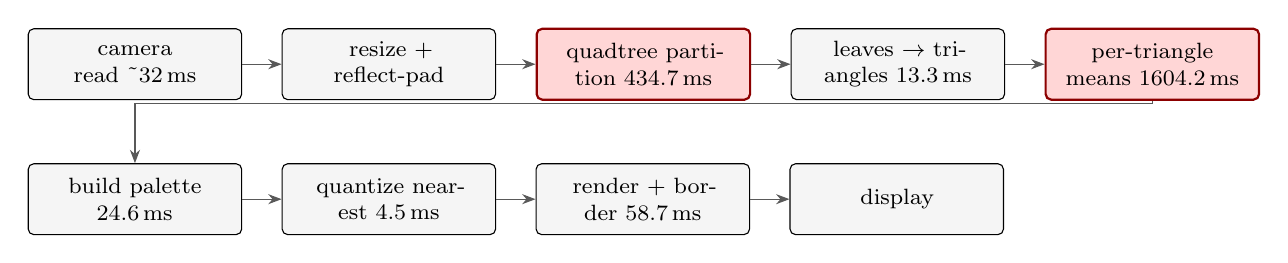
\begin{tikzpicture}[
  font=\footnotesize,
  node distance=3mm and 5mm,
  stage/.style={draw, rounded corners=2pt, align=center, inner sep=3pt,
                text width=25mm, minimum height=9mm, fill=black!4},
  hot/.style={stage, fill=red!16, draw=red!55!black, thick},
  flow/.style={-{Stealth[length=1.7mm]}, draw=black!65, thin}
]
\node[stage]                          (a) {camera read \textasciitilde 32\,ms};
\node[stage, right=of a]              (b) {resize + reflect-pad};
\node[hot,   right=of b]              (c) {quadtree partition 434.7\,ms};
\node[stage, right=of c]              (d) {leaves $\rightarrow$ triangles 13.3\,ms};
\node[hot,   right=of d]              (e) {per-triangle means 1604.2\,ms};
\node[stage, below=8mm of a]          (f) {build palette 24.6\,ms};
\node[stage, right=of f]              (g) {quantize nearest 4.5\,ms};
\node[stage, right=of g]              (h) {render + border 58.7\,ms};
\node[stage, right=of h]              (i) {display};
\draw[flow] (a) -- (b);
\draw[flow] (b) -- (c);
\draw[flow] (c) -- (d);
\draw[flow] (d) -- (e);
\draw[flow] (e) -- ++(0,-5mm) -| (f.north);
\draw[flow] (f) -- (g);
\draw[flow] (g) -- (h);
\draw[flow] (h) -- (i);
\end{tikzpicture}
\end{figure}

The baseline is measured at the full-quality config (quadtree,
$S_{\text{set}}=[1..32]$, $K=16$, kmeans\_lab, budget=9990, 640$\times$480,
scale=1.0):

\begin{table}[htbp]
\centering
\begin{tabular}{@{}l r r r@{}}
\toprule
\textbf{Stage} & \textbf{median ms} & \textbf{mean ms} & \textbf{Share}\\
\midrule
camera read                  & \textasciitilde32 & ---             & --- \\
quadtree\_partition          & 434.7 & 427.4 & 20\% \\
leaves\_to\_triangles        & 13.3  & 13.5  & 1\% \\
\textbf{triangle\_means\_bgr} & \textbf{1604.2} & \textbf{1595.3} & \textbf{75\%} \\
build\_palette               & 24.6  & 105.0 & 1\% \\
quantize\_nearest\_bgr       & 4.5   & 4.9   & 0.2\% \\
render\_triangles            & 58.7  & 58.4  & 3\% \\
\midrule
\textbf{frame total}         & \textbf{2140} & 2204 & \textbf{0.45 FPS} \\
\bottomrule
\end{tabular}
\caption{Task 4 measured baseline before optimisation (full-quality config,
640$\times$480, 9{,}990 bricks). The six processing stages sum to 2{,}140\,ms,
which is the frame total the FPS column is computed from; the $\sim$32\,ms
camera read is measured separately and is not included in that sum. The stage
shares are percentages of the 2{,}140\,ms processing total.}
\label{tab:baseline}
\end{table}

\texttt{triangle\_means\_bgr} dominates because per triangle it zeroes a
full-frame mask and calls \texttt{cv2.mean} --- cost is $O(T\cdot H\cdot W)$.
The per-triangle cost scales with image area (903\,\textmu s/triangle at
1706$\times$1279, 143\,\textmu s at 640$\times$480, 39\,\textmu s at
320$\times$240 --- area ratios 7.1$\times$ and 4.0$\times$ track the
per-triangle ratios 6.3$\times$ and 3.6$\times$, which is the
$O(T\cdot H\cdot W)$ prediction). Two cheap parameter levers alone reach
$\sim$9\,FPS (reduce scale to 0.4 and budget to 1000, $K=6$), so the optimisation
work had to beat \textbf{9\,FPS at 1000 triangles}, not the easier 0.45\,FPS. A
later correction established that \texttt{build\_palette} was not 12$\times$
slower. A 2-frame run made a one-time $\sim$0.5\,s warm-up look like a per-frame
cost (median of two samples is their mean); with 30-frame runs the stage is
3--25\,ms/frame. I learned not to read per-stage percentages off a run too short
for the statistic to mean anything. Frame counts per table: the 0.45-FPS
baseline is an 8-frame run; the corrected palette figures are 30-frame runs;
per-stage isolation figures are single-frame-repeat or 12-frame paired runs
(details in \texttt{docs/progress/Task4.md}).

\FloatBarrier
\FloatBarrier
\subsection{Camera capture and display}
\label{sec:t4-display}

\texttt{camera\_app.py} opens the real camera, runs the full pipeline per frame,
and shows a side-by-side window. I verified the display numerically against
\cpath{code/pics/task4/L1\_baseline/frame0001\_\{input,render,compare\}.png}:
the render has exactly 17 distinct colours ($K=16$ palette + 1 border colour);
the border $(60,60,60)$ covers 74{,}592\,px, or 24.3\% of the 640$\times$480
frame, which makes it the single most common colour in the render and measurably
affects metrics, so the render path is the only place a border is drawn; the
palette spans the full dark-to-bright range with a real spread of hues; and
overall contrast is broadly preserved (render std 62.1 vs input 70.4, measured on
the saved frames). One defect caught me during this stage: the HUD's FPS first
read its timestamp immediately after \texttt{cap.read()}, so it reported the
camera's own $\sim$33\,FPS no matter how slow the pipeline was. The timestamp is
now taken after all per-frame work, and the HUD, the headless log and the
benchmark share one measurement path.

\figfull{task4/L1_baseline/frame0001_compare}{A real camera frame side by
side with its triangle-brick render ($K=16$, 9{,}990-brick quality preset).
Input and render are shown together because a mosaic judged without its input
says nothing about fidelity.}{fig:task4frame}

\FloatBarrier
\FloatBarrier
\subsection{Meeting the real-time constraint}
\label{sec:t4-optimise}

\textbf{Step 1: mean colour.} The shipped \texttt{triangle\_means\_bgr} has a
real defect, not just a speed problem: \texttt{cv2.fillPoly} paints a one-pixel
fringe along the \emph{right} and \emph{bottom} edges of every triangle (pixels
whose centres belong to the neighbouring cell), so every Task 2/3 brick's colour
is contaminated by its bottom-right neighbours. The leak is up to 400\% on
size-1 bricks and around 8\% of pixels overall. I added two new implementations
in \texttt{code/brick\_means.py}:

\begin{table}[htbp]
\centering
\begin{tabular}{@{}l r r r r r@{}}
\toprule
\textbf{\texttt{--means}} & \textbf{FPS} & \textbf{means stage} & \textbf{whole frame} & \textbf{$\Delta$E2000} & \textbf{PSNR}\\
\midrule
mask (shipped)                & 0.41 & 1716\,ms & 2260\,ms & 9.947 & 14.90\,dB \\
\textbf{fast} (exact in-cell) & \textbf{1.35} & \textbf{20.8\,ms} & \textbf{532\,ms} & \textbf{8.633} & \textbf{15.33\,dB} \\
sample (9 interior pts)       & 1.47 & 5.2\,ms & 493\,ms & 10.244 & 14.87\,dB \\
\bottomrule
\end{tabular}
\caption{Mean-colour implementations: speed and quality
(640$\times$480, 9{,}990 bricks).}
\label{tab:means}
\end{table}

\texttt{fast} is 82$\times$ faster on the stage, 3.3$\times$ overall,
\emph{and} closer to the source ($\Delta$E 9.95 $\rightarrow$ 8.63) because it
averages only in-cell pixels. \texttt{sample} is fastest but worse than even the
leaky reference on small bricks (nothing to sample inside a 1--4\,px triangle).
The defect is not a corner case: over the real 4{,}995-cell partition the
reference averages 8.1\% foreign pixels (186{,}021 of 2{,}297{,}721), and
per-triangle means differ from the correct in-cell means by an average of $\sim$3.0
grey levels per channel (max 46.1). Every recorded Task 2/3 number inherits this
small directional bias, but cross-run comparisons are unaffected because all
runs used the same leaky reference; the corrected in-cell means are what the
report's Task 2/3 numbers would give if the fringe were absent --- a disclosed
limitation. (Quantified with \texttt{compare\_means} in
\texttt{code/brick\_means.py}; full numbers in
\cpath{docs/progress/Report\_prep\_assets.md} \S3.)

\textbf{Step 2: partition.} \texttt{quadtree\_partition} recomputed a numpy
region mean per split candidate. Two fixes: drop 4 dead SSE computations per
split (436 $\rightarrow$ 326\,ms), then replace numpy region means with
\textbf{summed-area tables} ($O(1)$ rectangle SSE), batched so the $\sim$160{,}000
small per-candidate calls collapse into one query per split. Isolated:

\begin{table}[htbp]
\centering
\begin{tabular}{@{}l r r r@{}}
\toprule
\textbf{Implementation} & \textbf{2000 bricks} & \textbf{5000 bricks} & \textbf{9990 bricks}\\
\midrule
ref (numpy)           & 80\,ms & 173\,ms & 326\,ms \\
sat (tables, batched) & 44\,ms & 69\,ms  & \textbf{107\,ms} \\
speedup               & 1.8$\times$ & 2.5$\times$ & \textbf{3.0$\times$} \\
\bottomrule
\end{tabular}
\caption{Partition implementation: summed-area tables vs numpy reference.}
\label{tab:partition}
\end{table}

The partition is \textbf{bit-identical} under \texttt{mse} priority (cell set and
size distribution match exactly), so no Task 3 result is invalidated. Caveat:
\texttt{edgef1} priority with the table impl uses a global Sobel map and is NOT
numerically equal to the recorded per-region-Sobel runs (median $\sim$2$\times$
relative difference near region edges); the recorded E\_priority numbers are
pinned to \texttt{docs/progress/Task3.md} and \texttt{metrics\_table.csv}, and
the code prints an explicit note when this combination is used. The conclusion
($\Delta$MSE beats Sobel priority) is robust under both implementations.

\textbf{Step 3: whole-pipeline analysis.} With means and partition fixed, the
frame is $\sim$216\,ms and the remaining bottlenecks are partition $\sim$107\,ms
($\sim$50\%, 1{,}565 greedy splits that add 4{,}695 cells to the 300-cell start
grid, with the cost dominated by numpy-call count rather than the arithmetic),
render $\sim$55\,ms ($\sim$25\%, $\sim$20{,}000 Python-to-cv2 crossings), palette
$\sim$23\,ms ($\sim$10\%, per-frame K-Means), and triangles $\sim$13\,ms. I
applied four optimisations (all exact unless noted). Optimisation A is a batched
render that groups up to $K$ \texttt{fillPoly} calls by colour plus one
\texttt{polylines}, taking render from 55\,ms to $\sim$8\,ms with \textbf{0
differing pixels}. Optimisation B precomputes split priorities by scoring all
$\sim$102k candidates up front so the greedy loop is pure Python; partition
drops from 107\,ms to $\sim$30\,ms and the leaves stay bit-identical.
Optimisation C changes the palette refresh cadence to rebuild every 10 frames,
keeping the palette byte-stable in between, which amortises palette from
22.0\,ms to 4.9\,ms per frame. Optimisation D vectorises
\texttt{leaves\_to\_triangles}, taking triangles from 13\,ms to $\sim$2\,ms.
Paired in-process benchmark (synthetic 640$\times$480, reps=5):

\begin{table}[htbp]
\centering
\begin{tabular}{@{}l r r l@{}}
\toprule
\textbf{stage} & \textbf{old} & \textbf{new} & \textbf{speedup}\\
\midrule
partition           & 72.3\,ms & 33.8\,ms & 2.14$\times$ \\
triangles           & 8.3\,ms  & 2.2\,ms  & 3.79$\times$ \\
render              & 28.1\,ms & 8.4\,ms  & 3.35$\times$ \\
palette (amortised) & 22.0\,ms & 4.9\,ms  & 4.47$\times$ \\
\midrule
\textbf{whole frame} & \textbf{129.0\,ms} & \textbf{59.5\,ms} & \textbf{2.17$\times$ ($\sim$16.8 FPS processing-only)} \\
\bottomrule
\end{tabular}
\caption{Whole-pipeline paired benchmark after optimisations A--D (synthetic
640$\times$480, reps=5).}
\label{tab:pipeline}
\end{table}

App-level before/after (same machine, same input): TOTAL 130.5 $\rightarrow$ 62.0\,ms
with $\Delta$E2000 11.014 == 11.014, PSNR 15.68 == 15.68, \textbf{0 pixels
differ}.

\textbf{Step 4: frame-to-frame jitter (root cause).} With the camera held still
the mosaic still flickered every frame. To find out why, I probed headlessly in
\texttt{code/task4\_verify.py}: the pipeline was driven on four synthetic
sequences (identical frames, noise $\sigma=2$, frozen geometry, and a
$+1.5$-brightness-per-frame ramp), and on each sequence the per-frame canvas
churn was measured both on ordinary frames and on the frames where the palette
rebuilds (every 10th). Churn here means the fraction of pixels whose maximum
channel change exceeds 8 grey levels. The probe results are the source for every
number in this step:

\begin{table}[htbp]
\centering
\begin{tabular}{@{}l l l@{}}
\toprule
\textbf{sequence} & \textbf{per-frame churn} & \textbf{on a palette-rebuild frame}\\
\midrule
identical frames         & 0.000\%      & \textbf{canvas 76.6\%} \\
noise $\sigma=2$         & 0.55--0.96\%  & \textbf{canvas 76.7\%} \\
noise, geometry frozen   & 0.31--0.59\%  & \textbf{canvas 76.7\%} \\
brightness drift         & 2.85--8.07\%  & \textbf{canvas 76.7\%} \\
\bottomrule
\end{tabular}
\end{table}

So ordinary frames churn by at most a few percent, but on the rebuild frame the
canvas jumps by 76.7\% of its pixels. Three independent causes came out of the
probe.

The dominant one is K-Means instability. A rebuild re-runs \texttt{cv2.kmeans}
from OpenCV's global RNG, which lands on a different local optimum each time, and
because every triangle's label is re-decided against the new palette, a different
optimum re-colours most of the canvas at once. Feeding identical pixels through
K-Means without re-seeding gave a max palette delta of \textbf{180} (the probe's
\texttt{pal\_d1} column); with a fixed seed, identical input collapses the delta
to 0, but two different noisy frames with the same seed still produced a delta
of \textbf{144}. Re-seeding alone does not solve this, so I had to attack the
rebuild itself rather than its random seed.

The second cause is that the pipeline had no temporal coherence anywhere.
Partition, means, and quantise were recomputed every frame from noisy pixels, so
sensor noise was moving near-tie split decisions on 3--5\% of cells per frame and
flipping labels near palette boundaries on roughly 3\% of cells. With nothing to
anchor the output, even a steady scene drifted.

The third cause is camera auto-exposure and white-balance drift, which amplifies
the other two. A 1.5/255-per-frame brightness ramp was enough to raise per-frame
canvas churn from about 0.5\% to 2.9--8.1\%. So even after I fixed K-Means and
added coherence, an unlocked camera exposure would still keep churning the
output.

\textbf{Step 5: the fix (A+B+C).} Fix A is to warm-start the palette from the
previous one, refining the previous local optimum instead of jumping to a new
one, plus a dead-band that discards a rebuild where no entry moves by more than
2 grey levels. Fix B is to reuse the partition when a keyframe signature says
the scene has not changed; static frames keep the same leaves, while means are
still re-extracted from the live pixels. Fix C is quantise hysteresis: a
per-triangle label memory keeps the previous label unless a different palette
entry wins by a relative margin. Measured (churn = fraction of pixels whose max
channel change exceeds 8 grey levels):

\begin{table}[htbp]
\centering
\begin{tabular}{@{}l r l@{}}
\toprule
\textbf{metric} & \textbf{before} & \textbf{after}\\
\midrule
palette delta on rebuild, identical input & \textbf{153} & \textbf{1} \\
steady per-frame churn, noise $\sigma=2$   & \textbf{2.400\%} & \textbf{0.064\%} (37.7$\times$ less) \\
rebuild-frame churn, identical frames     & 0.013\% & \textbf{0.000\%} \\
rebuild-frame churn, noise $\sigma=2$     & 0.029\% & \textbf{0.000\%} \\
app static TOTAL\,ms (temporal OFF $\rightarrow$ ON) & 68.9 & \textbf{27.5} \\
partition stage\,ms                       & 37.7 & \textbf{0.2} (reused) \\
\bottomrule
\end{tabular}
\caption{Frame-to-frame jitter fixes (temporal coherence A+B+C): before/after.}
\label{tab:jitter}
\end{table}

The rebuild-frame flash measured in Step 4 (76.7\% of pixels on every 10th frame)
is gone --- a rebuild is now a refinement, not a re-colouring; the continuous
crawl drops $\sim$38$\times$ on realistic sensor noise; and the partition stage
disappears on a static scene. Note the two palette-delta numbers: Step 4's
\textbf{180} is the palette-only micro-test (\texttt{pal\_d1} in the probe, no
re-seed), while Table~\ref{tab:jitter}'s \textbf{153} is the app-level
cold-vs-warm rebuild measured at the temporal layer --- they are two different
probes, and Table~\ref{tab:jitter} compares the fix to the second of them.

\textbf{Step 6: render reuse and row-run means (opt E).} Two remaining per-frame
costs on a static scene: means ($\sim$14\,ms) and render ($\sim$10\,ms). E1:
exact \textbf{row-run means} --- each triangle half is a contiguous pixel run per
row, so a per-row prefix-sum table answers a row's run in two lookups;
bit-identity is provable (exact integer sums $< 2^{24}$, so float32 holds them
exactly and addition order cannot change the value). \texttt{task4\_verify}
asserts $\max|\mathrm{diff}| = 0$: 14.2 $\rightarrow$ 7.7\,ms (1.85$\times$). E2:
\textbf{render reuse} --- the canvas is a pure function of
\texttt{(tri, labels, palette, shapes)}; when geometry is reused and
labels+palette are byte-identical, the cached canvas is the image, so rasterising
is skipped (10 $\rightarrow$ 0\,ms on a static scene; under noise it correctly
does not fire, because labels change). Stacked effect on a static scene: 68.9\,ms
baseline $\rightarrow$ \textbf{27.5\,ms} with temporal coherence (step 5)
$\rightarrow$ \textbf{11.4\,ms} with opt E as well, i.e. $\sim$6$\times$
overall, all exact reuse and no quality cost. Note that the 37.1\,FPS quoted in
step 8 below is the \emph{step-5} figure (1/27.5\,ms), measured before opt E
existed; the delivered static number is 11.4\,ms, about 88\,FPS. I have left both
in place because each is a real measurement of the build that existed at the
time, but they are not comparable and I should not have quoted 37\,FPS as the end
state.

\textbf{Step 7: display panel.} Two presentation defects fixed: the HUD
previously drew 14 lines on solid black boxes covering $\sim$35--40\% $\times$
30--35\% of the render pane (now three lines on one translucent panel,
$\sim$15\% $\times$ 3--4\%); and resizing a \texttt{WINDOW\_NORMAL} window
stretched the bricks (fixed by uniform letterbox scaling into the window's image
area, so OpenCV's stretch becomes the identity).

\textbf{Step 8: reuse freezes colour + camera AE/WB lock.} Even after A+B+C, a
static scene still showed residual colour churn (0.101\% of pixels/frame)
because means and quantize were still re-running every frame. The fix is, when
the partition is reused, also freeze the previous labels plus the canvas, which
makes an unchanged scene byte-identical frame to frame. I also locked the
camera's auto-exposure (\texttt{--lock-ae}, optionally at a fixed
\texttt{--exposure}) and its auto white-balance (\texttt{--lock-wb}, a separate
flag) because a steady exposure is what makes freezing colour safe rather than
stale. Both are opt-in flags, not preset behaviour --- the \texttt{quality}
preset sets only \texttt{scale}, \texttt{budget} and $K$, so a reader running the
default gets drifting exposure unless they pass the flags, and the same is true
of the failure case below. Measured: churn 0.101\% $\rightarrow$ \textbf{0.000\%},
static effective FPS 22.6 $\rightarrow$ \textbf{37.1}. I confirmed on the real
camera that the jitter is noticeably reduced and the fidelity is no worse.

\FloatBarrier
\FloatBarrier
\subsection{Behaviour across different content}
\label{sec:t4-content}

The same pipeline was run on seven camera snapshots of different content,
captured with \cpath{camera\_app.py --lock-ae --snapshot-dir
code/pics/task4/} (\texttt{snap\_000.png} \ldots \texttt{snap\_006.png}, each
pairing the raw frame on the left with its triangle-brick render on the right).
They cover two portraits under different lighting, a strongly textured keyboard,
a group of saturated luggage items, a low-light desk lamp, a curtain against
window light, and a near-overexposed wall.

\figfull{task4/L2_contact_sheet}{Seven camera snapshots of different
content, each pairing the raw frame (left) with its triangle-brick render
(right), composed by \cpath{code/task4\_l2\_contact\_sheet.py} into
\cpath{code/pics/task4/L2\_contact\_sheet.png}. The adaptive tessellation puts
small bricks on detail and large bricks on flat regions in every scene; the same
configuration runs on all of them.}{fig:contactsheet}

The renders hold up across content types. In the two portrait frames
(\texttt{snap\_000} front-lit against a flat wall, \texttt{snap\_001} backlit
through a sheer curtain) the glasses outline, face contour and hair edge survive
as dense fine bricks, with one consistent artefact: the cool-toned indoor light
comes out warmer than the input, which a white-balance pass would fix. The
keyboard (\texttt{snap\_002}) drives small bricks across the whole key field
while the desk stays in large flat cells. The luggage scene (\texttt{snap\_003})
is the one that separates palette from geometry: sage-green, teal and maroon
cases against a warm wooden floor give the 16-colour palette genuinely distinct
hues to separate, and the bricks shrink onto the bag seams and zips while the
near-flat wall behind stays coarse. The lamp scene (\texttt{snap\_004}) is the
hardest lighting case, a blown-out bulb against a barely lit wall, and the lamp
body and light source are still legible because the saturated region gets the
finest cells. In the curtain frame (\texttt{snap\_005}) the folds and the window
grid are carried by brick density rather than by colour. The last frame
(\texttt{snap\_006}) is the one genuine failure: the source is a nearly uniform
bright wall whose switch and light bar are already close to blown out, and at
that contrast the mosaic loses the subject almost entirely. That is the expected
behaviour of a fixed palette under clipping, and it is why I capture with
\texttt{--lock-ae} rather than letting the camera normalise the exposure away ---
a locked exposure is what makes the fixed-palette assumption safe, and it is a
deliberate flag rather than preset behaviour.

The palette is reused across frames within tolerance
(\texttt{--palette-refresh 10}); no per-scene recalibration was needed.

\FloatBarrier
\FloatBarrier
\subsection{Robustness in a real scenario, and summary of the measured changes}

Robustness in a real scenario comes down to four distinct failure modes, and I
answer each with a measurement rather than an intention. The evidence lives in
the sections named.

\begin{itemize}
\item \textbf{Does it stay within the assignment's limits on unseen content?}
  The partitioner cannot exceed the budget by construction --- the quadtree
  guard is \texttt{while heap and n\_tri + 6 <= max\_triangles}, and
  \texttt{region\_merge\_partition} raises rather than return an over-budget
  partition. The PDF's other hard constraint, no gaps and no overlaps, is
  verified rather than argued: \texttt{code/verify\_coverage.py} checks all three
  delivered tessellations and finds cells distinct and grid-aligned, each cell's
  two triangles satisfying the exact area identity
  $\mathrm{area}(a) + \mathrm{area}(b) = s^{2}$, and \textbf{0 uncovered
  pixels} in the rasterised crop (Section~1).
\item \textbf{Does it survive a deadline?} Measured per-stage and paired
  before/after throughout Section~\ref{sec:t4-optimise}, from 2{,}140\,ms down to
  59.5\,ms per moving frame, with the spatial optimisations exact to 0 differing
  pixels.
\item \textbf{Does it stay visually stable frame to frame?} The temporal layer
  and its measured churn numbers are in Section~\ref{sec:t4-optimise} step 8;
  churn on a static scene goes 0.101\% $\rightarrow$ 0.000\% of pixels. The
  conditions that make this safe --- a locked exposure --- are stated there rather
  than assumed, and I flag that the flags are opt-in.
\item \textbf{Does it behave on content I did not design for?}
  Section~\ref{sec:t4-content} runs seven scenes spanning portraits, hard
  texture, saturated colour, low light, backlit fabric and a near-overexposed
  wall, and reports the one configuration that fails rather than only the six
  that work.
\end{itemize}

Where robustness is \emph{not} established, I would rather say so: this is a
single camera on a single machine (Section~\ref{sec:conclusion}), the test
content is one image for Tasks 2--3, and the temporal layer deliberately trades a
small amount of fidelity for stability.

Every optimisation I made in Section~\ref{sec:t4-optimise} is a paired
before/after with stage\,ms, whole-frame FPS, $\Delta$E/PSNR, and a pixel-diff
check, so each change is documented against the measurement that motivated it.
The headline reads cleanly only when each number's measurement conditions are
attached. With that in mind, and separating three different things that are easy
to conflate:

\begin{itemize}
\item \textbf{Per-frame cost at the full quality config, moving input.}
  2{,}140\,ms before optimisation $\rightarrow$ \textbf{59.5\,ms}, i.e.
  $\sim$16.8\,FPS processing-only on synthetic frames
  (Table~\ref{tab:pipeline}). An intermediate build, after the two
  $O(T\cdot H\cdot W)$/per-candidate fixes but before the render and means work,
  measured $\sim$215\,ms ($\sim$4.6\,FPS); that was a waypoint, not the delivered
  figure.
\item \textbf{The same pipeline on a static scene.} 68.9 $\rightarrow$
  \textbf{11.4\,ms} ($\sim$88\,FPS) with exact spatial reuse. The 37.1\,FPS in
  step 8 is the step-5 measurement of this (27.5\,ms) and is superseded.
\item \textbf{The camera's own ceiling.} Its 31--33\,FPS read-back is a separate
  limit and is not something these optimisations change.
\end{itemize}

The spatial optimisations are exact, with 0 differing pixels on identical input.
The temporal layer (palette cadence, warm-start, dead-band, hysteresis,
freeze-on-reuse) is a deliberate frame-to-frame approximation made for stability,
and it does trade a small amount of fidelity for that stability, which is why
paired ratios, not absolute FPS, are the trustworthy numbers here (see
Section~\ref{sec:t4-baseline}).

\FloatBarrier
\FloatBarrier
\subsection{Problems found and solved (Task 4)}

The 0.45\,FPS baseline came from two main offenders: the
$O(T\cdot H\cdot W)$ means stage and the per-candidate numpy means inside the
partition (Section~\ref{sec:t4-baseline}). I solved them with in-cell means, SAT
tables, batched render, precomputed priorities, palette cadence, and vectorised
triangles, all detailed in Section~\ref{sec:t4-optimise}.

A second issue was fringe-contaminated means, a latent bug in the shipped
reference implementation that also affected my Task 2/3 runs. The fix is in
Section~\ref{sec:t4-optimise} step 1, the measurement is in
Section~\ref{sec:t4-optimise}, and I disclosed the residual impact on the
recorded Task 2/3 numbers there as well.

K-Means palette instability was the third problem. The combination of a global
RNG and 10 restarts on near-degenerate data was flipping local optima between
frames (Section~\ref{sec:t4-optimise} step 4). I addressed it with warm-start
plus dead-band plus reuse plus AE/WB lock (Section~\ref{sec:t4-optimise} steps 5
and 8).

Two presentation defects also needed attention, namely the HUD FPS misreport and
the window stretch on resize. Their fixes are in
Section~\ref{sec:t4-display} and Section~\ref{sec:t4-optimise} step 7.

Finally, the \texttt{build\_palette} ``anomaly'' turned out to be a 2-sample
measurement artifact, not a real performance problem, as I worked out in
Section~\ref{sec:t4-baseline}.

\FloatBarrier
\FloatBarrier
\section{GenAI usage}

I used GenAI (PolyU GenAI and a general-purpose LLM) on every
GenAI-collaboration task. Across the three tasks I logged 17 prompts: 14 were
adopted, and 3 were rejected or rolled back after measurement. The role it
played, and the episodes that taught me the most about how it reasons, are
below; the per-task records live in \texttt{docs/progress/Task\{2,3,4\}.md}.

\FloatBarrier
\FloatBarrier
\subsection{How GenAI understood the tasks}

Three episodes from this work taught me the most about how the model actually
reasons.

The first is a case of correct-looking code with a wrong mental model (the Task 3
quadtree loop). My guard encoded ``split down to budget'', the opposite of what
it should have done. The code ran without error, and only a careful review of
intent (splitting increases the count) exposed it. The lesson for me was that
AI-generated code which merely executes still needs a sanity check against what
the code is supposed to do.

The second is the cost-diagnosis turn in Task 4. The AI correctly identified that
the bottleneck was Python-to-numpy call count rather than algorithmic
complexity, and its follow-up question about ``exact or approximate? state the
invariant'' set the tone for every later optimisation, which kept each one exact
by construction.

\FloatBarrier
\FloatBarrier
\subsection{A bias the model shares with most assistants}

The third episode is a bias seen most sharply in the Task 3 $S_{\max}=64$
episode. When I asked the model to pick $S_{\max}$, it reported ``64 is the clear
winner'' by leading with the four metrics where 64 won and demoting the single
regression ($\Delta$E2000) to a parenthetical. Only after I pushed back did it
break $\Delta$E down by region and find that the shadow area was materially worse
under 64. What I took from this: the model framed its answer to match the
hypothesis I had already implied, and did not volunteer that objective metrics
and human perception can invert. Section~\ref{sec:ai-bias} returns to this as the
most consequential pattern of the whole project.

\FloatBarrier
\FloatBarrier
\section{GenAI limitations and areas for improvement}
\label{sec:ai-limitations}

This section is my own assessment, because the limitations of the tool are not
visible in the code it produced but in the places where I had to stop trusting
it. Four patterns showed up repeatedly across the four tasks, and I have
arranged them by what they cost me: the bias that shaped my conclusions, the
unreliability of the code itself, the model's reluctance to go and look something
up, and a memory problem that grew with the size of the project.

\FloatBarrier
\FloatBarrier
\subsection{The bias that shaped my conclusions}
\label{sec:ai-bias}

The first and most consequential pattern is that a single agent in a single
conversation converges toward whatever the user has already said. I noticed it
when I proposed that raising $S_{\max}$ would give the quadtree more room for
fine splits, and the model immediately agreed, then designed an experiment that
could only demonstrate my hypothesis. It never asked whether the premise was worth
interrogating. The same bias reappeared when the results came in: the model
reported ``$S_{\max}$=64 is the clear winner'' by leading with the four metrics
where 64 won and demoting the single contradicting metric, $\Delta$E2000, to a
parenthetical. The contradicting analysis, that the shadow region is clearly
worse under 64, was only produced after I pushed back
(Section~\ref{sec:smax-tradeoff}). What concerns me most is the third variant,
where the model treated a metric verdict as a perceptual verdict. The four
objective metrics preferred 64; my own eyes preferred 32; the model had not
anticipated that these could disagree, and so it had no framework for noticing
when they did.

I was not getting a wrong answer; I was getting a fluent answer from a model
that had adopted my framing as its own, and in a single continuous session there
was nobody to notice. The practice that actually helped was structural rather
than clever prompting: late in the project I began running the same draft
through several independent review passes, each instructed to attack it from a
different angle, and letting them disagree. A second reader with no memory of how
the argument was constructed is much harder to seduce than the same reader
continuing a conversation.

\FloatBarrier
\FloatBarrier
\subsection{Generated code runs without being correct}
\label{sec:ai-code}

The second pattern is that generated code runs without being correct. The
quadtree in Section~\ref{sec:t3-results} is the clearest example: the split guard
was written as ``if the triangle count is under budget, return'' and the loop as
``split while over budget'', which is a coherent-looking encoding of the belief
that splitting reduces the count. It does the opposite. The code compiled, ran,
and produced a plausible-looking mosaic that quietly used 4{,}320 of its
9{,}990 bricks. Nothing raised an error; the only symptom was that my measured
edge-alignment score was slightly negative. I found it by re-reading what the
code was trying to do rather than what it said, and the same class of error
appeared twice more, in the merge-candidate alignment and in the grid-step scan.
The mitigation I adopted is the one this report has been demonstrating
throughout: treat every optimisation as a claim about invariants and write an
assertion that would fail loudly if the claim were wrong, rather than trusting
that correct-looking code is correct.

\FloatBarrier
\FloatBarrier
\subsection{The model will not go and look something up}

The third pattern is that the model will not go and look something up unless told
to, and when it does search it may not search thoroughly enough. It proposed
K-Means in Lab space for the palette without mentioning that
\texttt{cv2.kmeans} depends on a global RNG, so the palette is not reproducible
between runs. It recommended edge-density split priority without noting that
Sobel variance computed per region and computed globally differ near region
boundaries. In both cases the missing information would have changed how I ran
the experiment, and neither was volunteered. My own version of the problem was
subtler: not a fabricated fact, but a confidently recommended algorithm whose
main drawback I had to discover in the measurements myself.

\FloatBarrier
\FloatBarrier
\subsection{A context-memory problem that grew with the project}

The fourth pattern is a context-memory problem that showed up precisely because
this project grew long. As the report accumulated numbers, figures and
decisions, the assistant began to lose track of what had already been
established, and on several occasions it produced figures that contradicted data
it had itself recorded earlier, or that did not match the evidence on disk. When
I audited the final draft I found mismatches of exactly this kind: values that
disagreed with the numbers in the same report, image captions that described
content the file did not contain, and a couple of quantities that were simply
invented rather than measured. None of these came from malice and most were
plausible in isolation; they came from the model reasoning over a context too
long for it to hold every earlier claim and cross-check each new one against it.
The consequence is a rule I now apply without exception: for a report of this
size, every figure, image and code reference has to pass either an independent
cross-audit or a manual re-check against the underlying files, because the
model's own confidence is not a reliable signal of whether a number is real.

What I would change for a future project is mostly about process rather than
about the model. I would put the adversarial review pass in from the start
rather than near the end, because it is the only mechanism I found that
reliably broke the agreement. I would require that any claim about a library
behaviour, a metric definition, or a published method be backed by a reference
or a run I performed myself, instead of being accepted because it sounded right.
And I would treat the assistant as a fast colleague whose proposals are
hypotheses to be tested, not as an authority whose output is merely to be
formatted. The parts of this project that worked were the parts where I was
checking: measuring before and after, asserting invariants, and being willing to
reject a suggestion after the numbers disagreed with it. The parts that failed
were the parts where I stopped checking.

\FloatBarrier
\FloatBarrier
\section{Conclusion}
\label{sec:conclusion}

I built a triangle-brick image-generation system that converts an image into
right-isosceles-triangle mosaics under a 10{,}000-brick budget, and worked
through all four assignment tasks.

In Task 2 I set up the tessellation and showed, with the 10-item metric suite,
that the colour-quantisation method matters less than the geometry. On this
luminance-dominated scene Otsu and K-Means came out close to each other, and the
naive fixed threshold won the edge metrics while losing the colour metrics. The
uniform grid's negative EPI quantified how much the geometry mismatches the
content.

Task 3 made the geometry adaptive (RDO quadtree) and the palette multi-colour
(K-Means-Lab). A 15-run sweep plus a rate-distortion study on \texttt{sky.jpg}
showed where the budget is best spent: $K=16$, $S_{\max}=32$ as the balanced
setting, $\Delta$MSE priority, quadtree. The $S_{\max}=32$-vs-64 result I
present as a two-sided trade-off rather than a single winner, for two reasons:
the sweep is single-image evidence, and a strong-hue scene may shift the
palette-method and $K$ rankings; and the sweep driver never seeds OpenCV's RNG,
so I measured its run-to-run $\Delta$E2000 spread at $\sim$0.4 and re-grounded the
colour-side comparisons whose $\Delta$E2000 gap was smaller than that on a
deterministic palette (Section~\ref{sec:smax-tradeoff}) or a seeded run
(Section~\ref{sec:chosen-config}). Being precise about what that floor does and
does not cover: each metric has its own floor, and Section~\ref{sec:t3-results}
lists every comparison against the matching one. The $K$ conclusion rests on a
$\Delta$E2000 gap of 2.34 against a 0.441 floor (5.3$\times$); the $S_{\max}$
and priority conclusions rest on structural gaps of 2.9$\times$ to 34$\times$
their own floors. Three comparisons do \emph{not} clear their floors and I have
said so rather than leaning on them: the colour side of the $S_{\max}$ trade-off,
the $S_{\max}$ 64-vs-128 step, and the colour side of the priority comparison.
The palette choice is the honest borderline --- 1.5$\times$ on $\Delta$E2000,
and Median-Cut is better on all four structural metrics --- and
Section~\ref{sec:chosen-config} sets out both sides of it instead of claiming a
win.

In Task 4 I turned the pipeline into a live camera loop and dealt with the
real-world problems the offline tasks never exercised: an
$O(T\cdot H\cdot W)$ mean stage that took 75\% of the frame, the AI-introduced
quadtree bug, a latent fringe defect, frame-to-frame jitter from unstable
K-Means and camera exposure drift, and a misleading HUD. I measured each before
and after; on a static scene the loop reaches 11.4\,ms per frame, about 88\,FPS
(headless, no camera read-back) through exact spatial reuse plus the declared
temporal-stability layer, against 2{,}140\,ms before any optimisation.

The pipeline's layered design, a shared geometry/colour/rendering core with one
decision layer per task, is what let the Task 4 optimisations be exact (0
differing pixels on identical input) while keeping the Task 2/3 geometry
reproducible. I declare the K-Means-Lab palette as run-to-run non-reproducible,
and I re-generate all headline numbers from
\cpath{code/pics/task3/best/*\_metrics.json} under a fixed seed.

The limitations I want to be honest about: a single test image for Task 2 and
Task 3, K-Means non-reproducibility (declared, bounded), and measurements from a
single machine for Task 4. The multi-scene testing (Section~\ref{sec:t4-content})
covers seven frames from one camera in one room, which is enough to show the
pipeline is not tuned to one image and not enough to claim generalisation.

\FloatBarrier
\FloatBarrier
\appendix
\FloatBarrier
\FloatBarrier
\section{Definitions of the evaluation metrics}
\label{app:metrics}

The image-quality numbers come from \texttt{code/brick\_metrics.py}; the timing
figures come from the \texttt{StageTimer} in \texttt{code/brick\_io.py}, and the
marginal-benefit figures from \texttt{code/task3\_marginal.py}. This appendix
covers the quality metrics, which are the ones whose meaning is easy to misread.
Each answers a different question about the same render, so the results can be
read without guessing.

\textbf{PSNR} (higher is better) is the peak signal-to-noise ratio between the
source and the render, computed per channel over the whole image and reported in
dB:
\[
  \mathrm{PSNR} = 10 \cdot \log_{10}\!\left( \frac{\mathrm{MAX}^{2}}{\mathrm{MSE}} \right),
  \qquad \mathrm{MAX} = 255
\]
It is the most familiar number here and the least discriminating, because a large
uniform colour shift costs it as much as a small structural error.

\textbf{SSIM} (higher is better) is the structural similarity index of Wang et
al.\ (2004), computed per channel on a sliding odd window of at most
7$\times$7 pixels (smaller only if an image dimension forces it) and averaged.
SSIM scores local contrast and luminance structure rather than raw pixel
agreement, so it penalises a blurred or structurally displaced render more than
a uniformly brightness-shifted one.

\textbf{MS-SSIM} (higher is better) is the mean of the SSIM score computed at
four progressively downsampled resolutions, using Gaussian-pyramid decimation
(\texttt{cv2.pyrDown}) between levels. Averaging across scales rewards structure
that survives decimation, so it is harder to satisfy with a good low-resolution
match and noise at the finest scale. This is a four-level arithmetic mean of
per-level SSIM, which is a simplification of the weighted formulation in Wang et
al.\ (2003); it is not the standard MS-SSIM weighting, and the numbers in this
report should be read as a multi-scale consistency check rather than as a
comparable-to-literature score.

\textbf{$\Delta$E2000} (lower is better) is the mean per-pixel CIEDE2000 colour
difference between source and render, computed after converting both from sRGB
through CIE Lab. It is the perceptual colour metric of the suite; roughly, a
value above 2 is a clearly visible colour difference, and the values in this
report (roughly 6 to 12) correspond to differences that are obvious on
side-by-side inspection.

\textbf{Edge F1, precision and recall} (higher is better) compare Canny edge
maps of the source and the render, both extracted with $\sigma = 2.0$. Because a
triangle boundary can sit a pixel away from a true edge and still look aligned,
each edge map is dilated by a 3-pixel tolerance and an edge pixel counts as
matched when it falls inside the other map's dilated version:
\[
\begin{aligned}
  \text{precision} &= \frac{|\text{render edges near a source edge}|}{|\text{all render edges}|} \\
  \text{recall}    &= \frac{|\text{source edges near a render edge}|}{|\text{all source edges}|} \\
  \mathrm{F1}      &= \frac{2 \cdot \text{precision} \cdot \text{recall}}{\text{precision} + \text{recall}}
\end{aligned}
\]
Note that the two ratios use different reference sets: precision asks how much of
what the mosaic drew is real structure, recall asks how much of the real
structure the mosaic reproduced. The dilation is one-sided, so a match just
outside the tolerance band is missed by both directions.

\textbf{EPI, edge-alignment correlation} (signed, higher is better) is the Pearson
correlation between the mean-centred Sobel gradient-magnitude fields of source
and render:
\[
  \mathrm{EPI} = \mathrm{corr}\!\left( |\nabla\, \text{source}|,\; |\nabla\, \text{render}| \right)
\]
It measures whether edge energy in the mosaic is co-located with edge energy in
the source, independent of overall intensity. A positive value means the two
agree about where the edges are; a negative value means they disagree, which in
this project is the signature of triangle boundaries that do not follow image
content. Because the magnitudes are sparse and heavy-tailed, a correct mosaic
still scores near zero, so the sign is the reliable part of the metric.

That has a consequence I should be explicit about, because the rest of the report
leans on EPI differences: because a good mosaic sits near zero,
\emph{magnitude comparisons between two good mosaics are not meaningful in
absolute terms} --- $+0.045$ and $+0.015$ are both ``close to zero and
positive'', and the ratio between them is not a quantity the metric defines.
Where I compare EPI between configurations (Sections~\ref{sec:t3-results} and
\ref{sec:chosen-config}) I use it as a sign-and-ordering signal on configurations
whose Edge F1 also moves in the same direction, never as a standalone effect
size, and I check each such claim against the 0.0021 run-to-run spread I
measured. The one comparison that rests on EPI's \emph{sign} rather than its size
is the Sobel-priority run, which is the only configuration in the sweep that
goes negative at all. The name is local to this report: it is a plain Pearson
correlation of Sobel magnitudes and is not the Edge-Preservation Index of the
image-fusion literature.

\textbf{Quantisation error} (lower is better) is the mean CIEDE2000 distance
between each triangle's own mean colour and the palette entry it was assigned. It
isolates the colour-quantisation half of the pipeline from the geometry half,
because it never looks at the rendered image. A high quantisation error with a
reasonable PSNR means the geometry is fine but the palette cannot represent the
image, which is the diagnostic that separated the $K$ sweep from the $S_{\max}$
sweep in Section~\ref{sec:t2}.

\textbf{Budget utilisation} is not a quality metric but the fraction of the
10{,}000 bricks the run consumed, $N / 10000$. All Task 3 runs sit at 0.998 to
0.999.

\textbf{Framing of the suite.} The metrics are deliberately not redundant. PSNR
and quantisation error see colour; SSIM and MS-SSIM see structure at one and
many scales; $\Delta$E2000 sees perceptual colour distance; edge F1 sees whether
detected edges coincide; EPI sees whether edge energy is co-located; and the
residual map in Fig.~\ref{fig:t2residual} shows where the two images disagree
rather than how much. The disagreements between them, rather than any single
score, are what produced the findings in Sections~\ref{sec:t2} and
\ref{sec:smax-tradeoff}.

\end{document}
